\documentclass[11pt]{article}
\usepackage[T1]{fontenc}
\usepackage[utf8]{inputenc}
\usepackage{lmodern,microtype}
\usepackage[margin=1in]{geometry}
\usepackage{amsmath,amssymb,amsthm,mathtools}
\usepackage{enumitem,booktabs,array,longtable}
\usepackage{xcolor,tikz,listings}
\usepackage[colorlinks=true,linkcolor=blue!45!black,citecolor=blue!45!black,urlcolor=blue!45!black]{hyperref}
\usepackage[nameinlink,noabbrev]{cleveref}
\hypersetup{pdftitle={Sharp Level-Set Dimensions for the Takagi--van der Waerden Functions},
pdfauthor={Zixuan Ye},pdfsubject={Sharp uniform dimension bounds and level-set structure},
pdfkeywords={Takagi function, van der Waerden function, level sets, Hausdorff dimension}}
\setlength{\emergencystretch}{1.5em}
\setlist{itemsep=2pt,topsep=4pt}
\newtheorem{theorem}{Theorem}[section]
\newtheorem{proposition}[theorem]{Proposition}
\newtheorem{lemma}[theorem]{Lemma}
\newtheorem{corollary}[theorem]{Corollary}
\theoremstyle{definition}
\newtheorem{definition}[theorem]{Definition}
\theoremstyle{remark}
\newtheorem{remark}[theorem]{Remark}
\newtheorem{example}[theorem]{Example}
\newcommand{\R}{\mathbb R}
\newcommand{\Z}{\mathbb Z}
\newcommand{\N}{\mathbb N}
\newcommand{\dimH}{\dim_{\mathrm H}}
\newcommand{\dimB}{\overline{\dim}_{\mathrm B}}
\newcommand{\HH}{\mathcal H}
\newcommand{\ind}{\mathbf 1}
\newcommand{\dist}{\operatorname{dist}}
\newcommand{\diam}{\operatorname{diam}}
\newcommand{\card}{\#}
\DeclareMathOperator{\supp}{supp}
\lstset{basicstyle=\ttfamily\footnotesize,columns=fullflexible,keepspaces=true,
breaklines=true,frame=single,rulecolor=\color{black!30},showstringspaces=false,
xleftmargin=3pt,xrightmargin=3pt,aboveskip=8pt,belowskip=8pt}
\title{\textbf{Sharp Level-Set Dimensions for the\\Takagi--van der Waerden Functions}}
\author{Zixuan Ye\thanks{Beijing National Day School, Beijing, China.}}
\date{October 2026}
\begin{document}
\maketitle
\begin{abstract}
The level sets of the Takagi--van der Waerden functions reflect a competition
between flat returns and crossings that may become flat only at later scales.
We prove a sharp upper bound of $1/2$ for the upper box dimension of every
level set, uniformly over all integer bases. The proof separates the two
sources of new flat pieces by their height residues and closes a coupled
counting recursion. It also gives an explicit covering bound and finite
$1/2$-dimensional Hausdorff measure. We construct dense families of levels
attaining the bound, including uncountably many irrational levels in base
three. For odd bases, we describe selected entire level sets and give a finite
classification on a dense arithmetic family. All general results have
analytic proofs; an accompanying exact-arithmetic script supplies finite
cross-checks.
\end{abstract}
\noindent\textbf{Keywords.} Takagi function; van der Waerden function; level
set; Hausdorff dimension; box dimension; self-affinity.
\section{Introduction}
For an integer $r\ge2$, let
\begin{equation}\label{eq:defT}
 T_r(x)=\sum_{n=0}^{\infty}\frac{\psi(r^nx)}{r^n},
 \qquad \psi(x)=\dist(x,\Z),\qquad x\in\R.
\end{equation}
Write $M_r=\max_{[0,1]}T_r$ and
$L_r(y)=\{x\in[0,1]:T_r(x)=y\}$.
Throughout, $\N=\{1,2,\ldots\}$ and
$a\bmod b=a-b\lfloor a/b\rfloor$ for real $a$ and $b>0$.
The case $r=2$ is the classical Takagi function; the family includes the
function studied by van der Waerden. Historical and analytic background is
surveyed in \cite{survey}.

The geometry of the level sets is considerably richer than the elementary
construction of these functions might suggest. Baba \cite{baba} determined
their maxima and maximizing sets. In even bases the maximal level set has
Hausdorff dimension $1/2$, whereas in odd bases the unique global maximizer
is $x=1/2$; see also \cite{allaartlevels}. Thus the odd-base maximal level
set does not reveal the largest dimension of a level set.
For the classical function, Maddock \cite{maddock} obtained an upper bound
of $0.668$, and de Amo, Bhouri, D\'iaz Carrillo and Fern\'andez-S\'anchez
\cite{deamo} proved the sharp bound $1/2$.
Allaart \cite{allaartdimension} developed a related method that counts
horizontal pieces and nonhorizontal crossings separately, including signed
binary Takagi functions. In \cite[Introduction]{allaartlevels}, the extension of
the bound to even bases was noted, while the corresponding odd-base
question was explicitly left unclear.

Another approach decomposes fibers into local level sets. Jiang, Ying
and Zhang \cite{jiang} extended this framework to every integer base and
computed the expected number of local level sets in a randomly chosen
fiber. Here we seek a uniform estimate that also controls exceptional
ordinates, where the largest dimensions occur.

This paper gives a self-contained counting proof for every integer base.
The difference between even and odd bases is retained in the recursion:
an odd base permits contributions from two adjacent height strips.
The decisive arithmetic fact is that these additional crossings cannot
create flat pieces at the same height residues as flat parents.
Consequently the two sources are compared by a maximum, rather than added.
This prevents delayed returns from increasing the exponential covering rate.

\subsection{Main results}
We use the convention $\dimH\varnothing=\dimB\varnothing=0$.
Set
\begin{equation}\label{eq:introgrid}
 \gamma_r=\begin{cases}1,&r\text{ even},\\2,&r\text{ odd},\end{cases}
 \quad \delta_m=r^{1-2m},\quad
 I_{m,j}=\left[\frac{j\delta_m}{2},\frac{(j+1)\delta_m}{2}\right]
 \quad(0\le j<2r^{2m-1}),
\end{equation}
and let $N_{r,2m}(y)$ be the number of these closed intervals whose
$T_r$-image contains $y$. A common endpoint is counted in each incident
interval.

\begin{theorem}[Uniform covers and dimensions]\label{thm:main}
For every integer $r\ge2$, every $y\in\R$ and every $m\ge1$,
\begin{equation}\label{eq:maincover}
 N_{r,2m}(y)\le
 2r^{m-1}+\frac{4(r^m-\gamma_r^m)}{r-\gamma_r}
 \le14r^{m-1}.
\end{equation}
In particular,
\begin{equation}\label{eq:mainDim}
 \dimH L_r(y)\le\dimB L_r(y)\le\frac12,
 \qquad
 \HH^{1/2}(L_r(y))\le
 \frac{2+4r/(r-\gamma_r)}{\sqrt{2r}}.
\end{equation}
Here Hausdorff measure is defined using powers of diameters, without a
normalizing factor.
\end{theorem}

The covering theorem is stronger than a dimension estimate alone: its
constant is uniform in the ordinate, and it controls the critical
Hausdorff measure. It does not assert that this measure is positive whenever
the dimension is $1/2$.

\begin{theorem}[Sharpness and irrational ordinates]\label{thm:sharpintro}
For every integer $r\ge2$, the set
$\{y\in[0,M_r]:\dimH L_r(y)=1/2\}$ is dense in $[0,M_r]$, and
\begin{equation}\label{eq:criticallevels}
 \dimH L_r\left(\frac{kr}{r^2-1}\right)=\frac12
 \quad\left(1\le k\le\left\lfloor\frac r2\right\rfloor\right).
\end{equation}
More generally, every flat partial-sum interval gives the family of
maximal-dimensional ordinates in \cref{eq:flatcode} below.
For $r=3$, if $E\subset\N$ has asymptotic density zero, then
\begin{equation}\label{eq:sparseintro}
 y_E=\frac38-\frac53\sum_{j\in E}81^{-j}
 \quad\text{satisfies}\quad \dimH L_3(y_E)=\frac12.
\end{equation}
In particular, every infinite $E\subset\{j^2:j\ge1\}$ gives an irrational
ordinate, and these choices give uncountably many distinct ordinates.
\end{theorem}

For odd bases, a further result describes entire level sets, including the
points outside a chosen Cantor subset. Fix an odd $r=2q+1\ge3$ and
$1\le k\le q$. Put $D=r^2-1$ and
\begin{equation}\label{eq:introarith}
 \mathcal A_{r,k}=
 \left\{y\in[0,M_r]:\text{ for some }m\ge0,\quad
 r^my\bmod1\in\left\{\frac{k}{D},\frac{kr}{D}\right\}\right\}.
\end{equation}

\begin{theorem}[Odd-base arithmetic structure]\label{thm:arithintro}
The set $\mathcal A_{r,k}$ is dense. For $y\in\mathcal A_{r,k}$, the level
set $L_r(y)$ is either finite or satisfies
$0<\HH^{1/2}(L_r(y))<\infty$. These two cases can be distinguished by a
finite exact procedure given a witness $m$ in \cref{eq:introarith}.
At $y=kr/D$, the entire level set consists of two reflected copies of a
Cantor set together with countably many isolated points. Moreover,
\begin{equation}\label{eq:criticalcountintro}
 N_{r,2m}\left(\frac{kr}{D}\right)
 =\frac{2(3r-1)r^{m-1}-4}{r-1}\qquad(m\ge1).
\end{equation}
\end{theorem}

An explicit description of $L_3(3/8)$ is given in
\cref{cor:ternarycondensation}. We also prove that the largest level-set
dimension of $T_r(x)+tx$ equals $1/2$ for every integer $t$
(\cref{cor:integer}). We do not claim a necessary and sufficient
classification of all maximal-dimensional ordinates, or a result for every
real slope.

\subsection{The counting idea and its scope}
On suitable half-$r$-adic intervals, $P_{2m}$ is affine with even integral
slope, and its endpoint heights lie in $\delta_m\Z$. After adding two
terms, the refinement is governed by a fixed integer staircase $W_r$.
Flat parents create new flat pieces at residues
$1,\ldots,\lfloor r/2\rfloor$ modulo $r$; nonflat parents create them only
at the complementary residues. If $a_m$ and $b_m$ denote the maximal flat
and crossing counts, respectively, this gives
\[
 a_{m+1}\le\max\{ra_m,b_m\},\qquad
 b_{m+1}\le ra_m+\gamma_rb_m.
\]
Since $r>\gamma_r$, a common invariant bound grows by $r$ per two scales.
The remaining tail is narrower than one height strip, so the two counts
also cover the actual level set.

The method follows the flat/crossing philosophy of
\cite[Section~3.1]{allaartdimension}; the integer profile, residue
separation and odd-base two-strip estimate are proved here for general
$r$. The historical reference to an odd-base question identifies a precise
earlier formulation, rather than asserting an exhaustive priority survey
of all later work. The main proofs below use no computer calculation.
The supplementary script checks finite instances and illustrative examples;
its role is specified in \cref{sec:verification}.

\section{Dimension conventions and an interval construction}
For a bounded $F\subset\R$, let $\mathcal N_\rho(F)$ be the least number
of intervals of length at most $\rho$ covering $F$. We use
\[
 \dimB F=\limsup_{\rho\downarrow0}
 \frac{\log\mathcal N_\rho(F)}{-\log\rho}.
\]
For $s>0$, let $\HH^s_\rho(F)$ be the infimum of
$\sum_i(\diam U_i)^s$ over countable covers of $F$ by sets of diameter at
most $\rho$, and set $\HH^s(F)=\lim_{\rho\downarrow0}\HH^s_\rho(F)$.
Hausdorff dimension is $\inf\{s>0:\HH^s(F)=0\}$.
An arbitrary subset of $\R$ may be replaced in a cover by its closed
interval hull, with the same diameter.
The definitions imply $\dimH F\le\dimB F$, invariance under nondegenerate
similarities, and that the Hausdorff dimension of a countable union is
the supremum of the dimensions. For the last assertion, apply countable
subadditivity of $\HH^s$ above that supremum. In particular a countable
set has dimension zero.

We record the elementary interval construction used for the lower bounds.
\begin{lemma}[Uniform interval construction]\label{lem:moran}
Let $0<\theta<1$. Starting from a closed interval of length $\ell_0>0$,
suppose every interval at step $n-1$ is replaced by $b_n\ge2$ closed
subintervals of length $\theta$ times its length, with disjoint interiors.
The number $b_n$ may depend on $n$, but is the same for every parent at that
step. Let $K$ be the nested intersection, $B_n=\prod_{j=1}^nb_j$ and
$\ell_n=\ell_0\theta^n$. Then
\begin{equation}\label{eq:morandim}
 \dimH K=\liminf_{n\to\infty}\frac{\log B_n}{-\log\ell_n}.
\end{equation}
If $b_n=b$ is constant and $s=\log b/(-\log\theta)$, then
$0<\HH^s(K)<\infty$.
\end{lemma}
\begin{proof}
The step-$n$ cover gives the upper bound in \cref{eq:morandim} by taking
a subsequence realizing the lower limit. Assign equal probabilities to the
children of each parent, and map an infinite sequence of choices to the
unique point of its nested intervals. This defines a probability measure
$\mu$ supported on $K$. Any point belongs to at most two step-$n$
intervals, so its mass is at most $2/B_n\to0$. Thus endpoints have zero
mass, and every step-$n$ interval has mass $1/B_n$.
An interval $J$ of length $\rho\le\ell_n$ meets at most three step-$n$
intervals, because those intervals have equal length and disjoint interiors.
Consequently, if $\ell_{n+1}<\rho\le\ell_n$, then
$\mu(J)\le3/B_n$.
For $s$ strictly below the right side of \cref{eq:morandim}, there is a
constant $C_s$ such that $B_n^{-1}\le C_s\ell_n^s$ for all $n$. Hence
$\mu(J)\le3C_s\theta^{-s}\rho^s$ at small scales. Every interval cover
then has $s$-cost at least $(3C_s\theta^{-s})^{-1}$, by summing the measure
inequality; so $\dimH K\ge s$. Let $s$ increase to the lower limit.
For constant $b_n=b$, the same argument works at the critical exponent,
while $B_n\ell_n^s=\ell_0^s$ bounds the critical Hausdorff measure above.
\end{proof}

\section{An integer refinement profile}\label{sec:profile}
Throughout the proof of the upper bound, $r\ge2$ is an arbitrary fixed
integer. Let
\[
 P_n(x)=\sum_{i=0}^{n-1}r^{-i}\psi(r^ix).
\]
Uniform convergence and positivity give
\begin{equation}\label{eq:tail}
 0\le T_r(x)-P_n(x)\le\frac{r^{1-n}}{2(r-1)}.
\end{equation}
All breakpoints of $P_{2m}$ lie on the grid of \cref{eq:introgrid}.

\begin{lemma}[Integral heights and even slopes]\label{lem:grid}
The function $P_{2m}$ is affine on each $I_{m,j}$, its slope there is an
even integer, and its endpoint values belong to $\delta_m\Z$.
\end{lemma}
\begin{proof}
Put $n=2m$ and $D=2r^{n-1}$. At an endpoint $j/D$,
\begin{equation}\label{eq:endpointinteger}
 D P_n(j/D)=\sum_{d=0}^{n-1}
 \min\{j\bmod(2r^d),\,2r^d-(j\bmod(2r^d))\}.
\end{equation}
Every summand is an integer with the parity of $j$, and $n$ is even.
Thus this sum is even, which proves the height assertion because
$D=2/\delta_m$. On each cell the slope is a sum of $2m$ signs $\pm1$.
\end{proof}

Write $q=\lfloor r/2\rfloor$ and $v=\lceil r/2\rceil$.
For an integer $z$, let $\alpha\in\{0,\ldots,2r-1\}$ be its residue
modulo $2r$, and define
\begin{equation}\label{eq:Wdef}
 W_r(z)=\frac{\min\{\alpha,2r-\alpha\}+(\alpha\bmod2)}2.
\end{equation}
It is a $2r$-periodic integer staircase, with
\begin{equation}\label{eq:Wshape}
 W_r(\alpha)=\begin{cases}
 \lceil\alpha/2\rceil,&0\le\alpha\le r,\\
 r-\lfloor\alpha/2\rfloor,&r\le\alpha\le2r.
 \end{cases}
\end{equation}
In particular $0\le W_r\le v$ and successive differences belong to
$\{-1,0,1\}$.

\begin{lemma}[Two-scale profile]\label{lem:profile}
On a parent $I_{m,j}$, suppose the left endpoint value of $P_{2m}$ is
$a\delta_m$ and its slope is $2s$, with $a,s\in\Z$. After subdivision
into $r^2$ children, the $d$th new endpoint has $P_{2m+2}$-height, in units
of $\delta_{m+1}$,
\begin{equation}\label{eq:profile}
 V_d=r^2a+s d+W_r(r^2j+d),\qquad0\le d\le r^2.
\end{equation}
On a nonflat parent, $P_{2m+2}$ is monotone. The new two-term contribution
lies everywhere between $0$ and $v\delta_{m+1}$.
If $r$ is even, $P_{2m+2}$ and $P_{2m}$ agree at both parent endpoints.
\end{lemma}
\begin{proof}
Put $n=2m$ and $z=r^2j+d$. The new endpoint is
$x=z/(2r^{n+1})$. Its old affine height, divided by $\delta_{m+1}$, is
$r^2a+sd$. The two new terms contribute
\[
 r\psi\left(\frac{z}{2r}\right)+\psi(z/2)=W_r(z),
\]
which proves \cref{eq:profile}. Each child is an affine piece, and its
endpoint increment is $s+W_r(z+1)-W_r(z)$. If $s\ne0$, all such increments
have the sign of $s$ or are zero. The bound on the new contribution holds
at all fine endpoints by \cref{eq:Wshape}, and between endpoints by
affinity. Finally, for even $r$, both $r^2j$ and $r^2(j+1)$ are multiples
of $2r$, so the endpoint contributions vanish.
\end{proof}

The two endpoint contributions in an odd base alternate between $0$ and
$v\delta_{m+1}$. This is the precise place where an adjacent old height
strip can contribute to a new crossing.

\section{Flat pieces, crossings, and residue separation}\label{sec:counts}
For $h\in\Z$, define
\begin{align*}
 A_m(h)&=\card\{j:P_{2m}|_{I_{m,j}}\equiv h\delta_m\},\\
 B_m(h)&=\card\{j:P_{2m}|_{I_{m,j}}\text{ is nonconstant and }
 P_{2m}(I_{m,j})\cap(h\delta_m,(h+1)\delta_m)\ne\varnothing\}.
\end{align*}
Let $a_m=\max_hA_m(h)$ and $b_m=\max_hB_m(h)$.
By \cref{lem:grid}, a nonflat cell counted by $B_m(h)$ contains the whole
open strip in its image. All counts refer to cells, including cells in a
longer flat interval, rather than to maximal affine pieces.

\begin{lemma}[Children of a flat parent]\label{lem:flatparent}
A flat parent at height $a\delta_m$ produces exactly $r$ flat children at
each height $(r^2a+k)\delta_{m+1}$, $1\le k\le q$. It also produces
exactly $r$ nonflat children crossing each fine strip with index
$r^2a+\ell$, $0\le\ell<v$. There are no other contributions.
\end{lemma}
\begin{proof}
With $s=0$, \cref{eq:profile} follows $r$ consecutive half-periods of $W_r$.
The starting phase is $0$ or $r$ modulo $2r$. Each half-period has length
$r$ and, by \cref{eq:Wshape}, has one horizontal step at each height
$1,\ldots,q$ and one nonhorizontal step across each band
$(\ell,\ell+1)$, $0\le\ell<v$. For even $r$, the two horizontal steps at
the peak lie on opposite sides of a half-period boundary; they are still
two distinct cells. The stated counts follow.
\end{proof}

\begin{lemma}[Children of a nonflat parent]\label{lem:nonflatparent}
A nonflat parent contributes at most one nonflat child to a fixed open
fine strip and at most one flat child to a fixed fine height. If it
contributes a flat child of height index $K$, then
\begin{equation}\label{eq:residueexclusion}
 K\bmod r\notin\{1,\ldots,q\}.
\end{equation}
\end{lemma}
\begin{proof}
By \cref{lem:profile}, the refined function is monotone on the parent.
The integer endpoints of any nonflat child force its image to contain an
entire open fine strip as soon as it intersects that strip. Two children
in monotone order cannot both contain that same open strip.

A flat child is possible only for $s=1$ or $s=-1$. Equal-sign nonzero
steps of $W_r$ are never adjacent, by \cref{eq:Wshape}. Hence flat children
of this parent are separated by a nonzero increment, so their heights are
distinct. To check the residue, put $z=r^2j+d$ and
$\alpha=z\bmod2r$; then $d\equiv\alpha\pmod r$.
For $s=1$, flatness requires a downward step of $W_r$, so $\alpha$ is odd
and $r\le\alpha\le2r-1$. Thus
\[
 K\equiv d+W_r(z)\equiv(\alpha+1)/2\pmod r,
\]
whose representative lies in $\{q+1,\ldots,r\}$.
For $s=-1$, flatness requires an upward step: $\alpha$ is even and
$0\le\alpha<r$. In that case
\[
 K\equiv-d+W_r(z)\equiv-\alpha/2\pmod r.
\]
Since $0\le\alpha/2\le v-1$, these residues lie in
$\{0,q+1,\ldots,r-1\}$. This proves \cref{eq:residueexclusion}.
\end{proof}

\begin{figure}[tb]
\centering
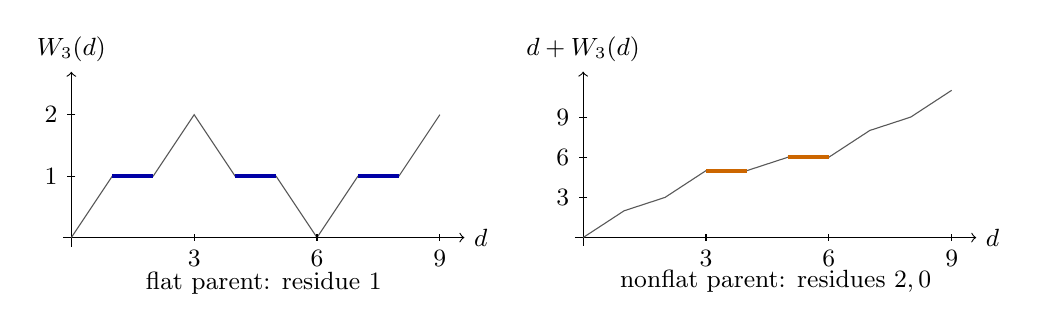
\begin{tikzpicture}[font=\small]
\begin{scope}[x=0.52cm,y=0.78cm]
\draw[->] (-0.2,0)--(9.6,0) node[right] {$d$};
\draw[->] (0,-0.15)--(0,2.7) node[above] {$W_3(d)$};
\draw[black!65] (0,0)--(1,1)--(2,1)--(3,2)--(4,1)--(5,1)--(6,0)--(7,1)--(8,1)--(9,2);
\draw[blue!65!black,line width=1.5pt] (1,1)--(2,1) (4,1)--(5,1) (7,1)--(8,1);
\foreach \x in {3,6,9}{\draw (\x,0.05)--(\x,-0.05) node[below] {\x};}
\foreach \y in {1,2}{\draw (0.1,\y)--(-0.1,\y) node[left] {\y};}
\node at (4.7,-0.75) {flat parent: residue $1$};
\end{scope}
\begin{scope}[xshift=6.5cm,x=0.52cm,y=0.17cm]
\draw[->] (-0.2,0)--(9.6,0) node[right] {$d$};
\draw[->] (0,-0.6)--(0,12.4) node[above] {$d+W_3(d)$};
\draw[black!65] (0,0)--(1,2)--(2,3)--(3,5)--(4,5)--(5,6)--(6,6)--(7,8)--(8,9)--(9,11);
\draw[orange!80!black,line width=1.5pt] (3,5)--(4,5) (5,6)--(6,6);
\foreach \x in {3,6,9}{\draw (\x,0.23)--(\x,-0.23) node[below] {\x};}
\foreach \y in {3,6,9}{\draw (0.1,\y)--(-0.1,\y) node[left] {\y};}
\node at (4.7,-3.3) {nonflat parent: residues $2,0$};
\end{scope}
\end{tikzpicture}
\caption{Two ternary local profiles in the even phase, after subtracting
the coarse height. Marked horizontal segments occur at height $1$ for a
flat parent, and at heights $5,6$ for a parent of half-slope $s=1$.
The incompatible residues persist at every scale.}\label{fig:profile}
\end{figure}

\begin{proposition}[Coupled recursion]\label{prop:recursion}
For $m\ge1$,
\begin{equation}\label{eq:recursion}
 a_{m+1}\le\max\{ra_m,b_m\},\qquad
 b_{m+1}\le ra_m+\gamma_rb_m.
\end{equation}
More precisely, if $K=r^2h+\ell$ with $0\le\ell<r^2$, then
\begin{equation}\label{eq:Bpointwise}
 B_{m+1}(K)\le rA_m(h)\ind_{\{\ell<v\}}+B_m(h)
 +\ind_{\{r\text{ odd}\}}B_m(h-1).
\end{equation}
\end{proposition}
\begin{proof}
Consider first flat children at height $K\delta_{m+1}$.
If $K\bmod r\in\{1,\ldots,q\}$, only flat parents contribute, by
\cref{lem:nonflatparent}. The contribution is $rA_m(h)$ when
$1\le\ell\le q$, and zero otherwise.
For the complementary residues, only nonflat parents contribute, each at
most once. Here $\ell=0$ or $\ell\ge q+1$.
On a flat child the old value is the new constant minus a contribution in
$[0,v\delta_{m+1}]$.
If $\ell=0$, these old values lie in
$((h-1)\delta_m,h\delta_m]$; since the old function is nonconstant on
the child, the parent crosses strip $h-1$.
If $\ell\ge q+1$, then $v\le q+1$ gives old values in
$[h\delta_m,(h+1)\delta_m)$, some strictly above $h\delta_m$; the parent
crosses strip $h$.
Thus these contributions are bounded by one of $B_m(h-1),B_m(h)$.
The two sources of flat children occupy disjoint residues, proving the
first inequality in \cref{eq:recursion}.

Now consider a fine open strip of index $K$. Flat parents contribute
$rA_m(h)\ind_{\{\ell<v\}}$ by \cref{lem:flatparent}.
Every nonflat parent contributes at most one nonflat child.
For odd $r$, a point in the fine strip has old height in
\[
 ((K-v)\delta_{m+1},(K+1)\delta_{m+1})
 \subset((h-1)\delta_m,(h+1)\delta_m).
\]
The parent's nonconstant affine image has integer grid endpoints, so it
crosses strip $h-1$ or strip $h$. Their union has at most
$B_m(h-1)+B_m(h)$ parents.
For even $r$, the refined function is monotone on a nonflat parent and
keeps its two endpoint values. Its image therefore equals the old affine
image. The fine strip lies in the old open strip $h$, so only $B_m(h)$
parents are needed. This proves \cref{eq:Bpointwise}; taking maxima gives
the second inequality in \cref{eq:recursion}.
\end{proof}

\begin{proposition}[Explicit counting bounds]\label{prop:counts}
For every $m\ge1$,
\begin{equation}\label{eq:abexplicit}
 a_m=2r^{m-1},\qquad
 b_m\le\frac{2(r^m-\gamma_r^m)}{r-\gamma_r}.
\end{equation}
\end{proposition}
\begin{proof}
The two half-periods of $P_2$ show $a_1=b_1=2$.
Because $r-\gamma_r\ge1$, the bounds at step $m$ imply
\begin{align*}
 a_{m+1}&\le\max\left\{2r^m,
 \frac{2(r^m-\gamma_r^m)}{r-\gamma_r}\right\}\le2r^m,\\
 b_{m+1}&\le2r^m+\frac{2\gamma_r(r^m-\gamma_r^m)}{r-\gamma_r}
 =\frac{2(r^{m+1}-\gamma_r^{m+1})}{r-\gamma_r}.
\end{align*}
This proves the upper bounds by induction. Starting with the two flat
cells at height $1/r$ and always choosing label $k=1$ in
\cref{lem:flatparent} gives $2r^{m-1}$ flat cells at a common height.
Thus the bound for $a_m$ is exact.
\end{proof}

The invariant behind this induction is also useful conceptually. If
$c=r/(r-\gamma_r)$, then $c\le r$ and the bound
$(a,b)\le P(1,c)$ is sent by \cref{eq:recursion} to at most
$rP(1,c)$. In particular, the extra odd-base coefficient $2$ remains
compatible with the covering rate $r$, even at the smallest odd base $3$.

\section{Actual level sets and maximal dimension}\label{sec:upper}
\begin{lemma}[A tail-sensitive cover]\label{lem:cover}
For every $y\in\R$, with $h=\lfloor y/\delta_m\rfloor$,
\begin{equation}\label{eq:coverAB}
 N_{r,2m}(y)\le A_m(h)+B_m(h-1)+B_m(h).
\end{equation}
\end{lemma}
\begin{proof}
By \cref{eq:tail}, a point with $T_r(x)=y$ has
\[
 P_{2m}(x)\in[y-\eta\delta_m,y],\qquad
 \eta=\frac1{2(r-1)}<1.
\]
This interval contains at most one grid height, necessarily $h\delta_m$.
Thus flat cells are bounded by $A_m(h)$.
For a nonflat cell, write its image endpoints as $a\delta_m,b\delta_m$
with integers $a<b$. If its image meets that interval, then
$a\le y/\delta_m<h+1$ and $b\ge y/\delta_m-\eta>h-1$.
Hence $a\le h$ and $b\ge h$. If $b=h$, it crosses strip $h-1$; if
$b\ge h+1$, it crosses strip $h$. This includes contacts at closed cell
endpoints and ordinates that are themselves grid heights.
\end{proof}

\begin{proof}[Proof of \cref{thm:main}]
Combine \cref{eq:coverAB,eq:abexplicit} to obtain the first bound in
\cref{eq:maincover}. Since $r/(r-\gamma_r)\le3$, the second bound follows.
The participating cells cover $L_r(y)$ and have length
$\ell_m=1/(2r^{2m-1})$. Their number is $O(r^m)$, so
\[
 \limsup_{m\to\infty}
 \frac{\log\mathcal N_{\ell_m}(L_r(y))}{-\log\ell_m}\le\frac12.
\]
Successive lengths have fixed ratio $r^2$; using the next finer cover
between these lengths proves the full upper box bound.
The Hausdorff bound follows.
Finally, the critical Hausdorff covering cost is at most
$N_{r,2m}(y)\sqrt{\ell_m}$. Taking the limit in the explicit first
bound of \cref{eq:maincover} gives the measure estimate in
\cref{eq:mainDim}.
\end{proof}

\subsection{Flat-return families}\label{sec:flatfamilies}
Call a half-$r$-adic cell $I$ \emph{flat of level $n$} if $P_n$ is
constant on $I$, where $n\ge1$ and $I$ has length $1/(2r^{n-1})$. Its level $n$ is
necessarily even. If $P_n|_I=c$, then \cref{lem:flatparent} gives, for each
$k\in\{1,\ldots,q\}$, exactly $r$ flat two-step descendants at height
$c+k/r^{n+1}$.

\begin{proposition}[Maximal-dimensional height codes]\label{prop:flatcodes}
For every such $I,c$ and every sequence $k_i\in\{1,\ldots,q\}$, put
\begin{equation}\label{eq:flatcode}
 y=c+\sum_{i=1}^{\infty}\frac{k_i}{r^{n+2i-1}}.
\end{equation}
Then $I\cap L_r(y)$ contains a compact set $K$ with
$0<\HH^{1/2}(K)<\infty$. Consequently $\dimH L_r(y)=1/2$.
For fixed $I$, the set of coded ordinates has dimension
$\log q/(2\log r)$, interpreted as zero when $q=1$.
\end{proposition}
\begin{proof}
At step $i$, retain all $r$ flat two-step children of label $k_i$ in every
retained interval. After $m$ steps there are $r^m$ intervals of length
$|I|r^{-2m}$, with disjoint interiors, on which $P_{n+2m}$ has the common
value
$c+\sum_{i=1}^m k_i/r^{n+2i-1}$.
The tail tends uniformly to zero, so their nested intersection is contained
in $L_r(y)$. Apply \cref{lem:moran} with $b=r$ and $\theta=r^{-2}$, and
then \cref{thm:main}.
The ordinates in \cref{eq:flatcode} are an affine image of
$\{\sum_{i\ge1}k_i(r^2)^{-i}:1\le k_i\le q\}$.
For $q\ge2$, its $q$ first-level interval hulls have disjoint interiors
and a positive gap, so the same lemma gives the stated dimension.
For $q=1$ it is a singleton.
\end{proof}

\begin{proof}[Proof of the first assertions of \cref{thm:sharpintro}]
Take $I=[(2k-1)/(2r),k/r]$, where $P_2=k/r$, and keep the constant label
$k$. Formula \cref{eq:flatcode} sums to $kr/(r^2-1)$, giving
\cref{eq:criticallevels}.

Every nonempty open subinterval $U$ of $[0,1]$ contains a flat cell.
Indeed choose a sufficiently small half-$r$-adic cell inside $U$.
Its partial-sum slope is an integer. The next summand has both derivative
signs among its $r$ children; select the sign that reduces the absolute
slope by one. Repeating reaches zero after finitely many steps.
Apply \cref{prop:flatcodes} inside that flat cell. Shrinking $U$ to an
arbitrary point and using continuity of $T_r$ proves density of the coded
maximal-dimensional ordinates throughout its range.
The irrational assertions are proved in \cref{sec:sparse}.
\end{proof}

\section{Odd bases: exact ranges and arithmetic rigidity}\label{sec:odd}
In this section $r=2q+1\ge3$ is odd. Put $A=r/(r-1)$ and define the
half-graph and its integer tilts by
\[
 f(u)=2T_r(u/2),\qquad f_t(u)=f(u)+tu\quad(0\le u\le1, t\in\Z).
\]
Since $r^n/2$ is a half-integer, $T_r(1/2)=A/2$. The termwise upper bound
in \cref{eq:tail} shows $M_r=A/2$. Also
$T_r(1-x)=T_r(x)$. The identity
$\psi(v+1/2)=1/2-\psi(v)$ gives
\begin{equation}\label{eq:antisymmetry}
 f(u)+f(1-u)=A.
\end{equation}
Let $\tau:[0,1]\to[0,1]$ be the continuous tent map with $r$ laps,
whose inverse branches are
\begin{equation}\label{eq:branches}
 h_j(v)=\frac{b_j+\varepsilon_jv}{r},\quad
 b_j=j+(j\bmod2),\quad \varepsilon_j=(-1)^j,
 \qquad0\le j<r.
\end{equation}
Folding $ru/2$ by period one and reflection in the first-term identity
for $T_r$ gives $f(u)=u+r^{-1}f(\tau u)$. Therefore
\begin{equation}\label{eq:states}
 f_t(h_j(v))=z
 \quad\Longleftrightarrow\quad
 f_{\varepsilon_j(t+1)}(v)=rz-(t+1)b_j.
\end{equation}
We call $(t,z)$ a \emph{state}, and call it admissible if $z$ lies in
the range of $f_t$. Each inverse word gives a closed $r$-adic interval;
its orientation can be reversed.

\begin{lemma}[Exact tilted ranges]\label{lem:ranges}
For integer $t$, the range $R_t=f_t([0,1])$ is
\begin{equation}\label{eq:ranges}
 R_t=\begin{cases}
 [0,A+t],&t\ge0,\\
 [A-s-A/r^s,\ A/r^s],&t=-s,\ s\ge1.
 \end{cases}
\end{equation}
\end{lemma}
\begin{proof}
For $t\ge0$, the bounds $0\le f\le A$ and the endpoint values give the
answer by continuity. For $s\ge1$, the first $s$ summands of $f(u)$ are
each at most $u$, and the remaining tail is at most $A/r^s$. Thus
$f(u)-su\le A/r^s$, with equality at $u=r^{-s}$. Indeed the first $s$
summands equal $u$ there and the remaining half-graph equals $r^{-s}f(1)$.
Finally, \cref{eq:antisymmetry} implies
$f_{-s}(u)+f_{-s}(1-u)=A-s$, which determines the minimum.
Continuity supplies every intermediate value.
\end{proof}

Fix $1\le k\le q$ for the rest of this section, and put
\begin{equation}\label{eq:residues}
 D=r^2-1,\quad d=\frac{2k}{D},\quad z_*=rd,\quad
 S=(d+2\Z)\cup(z_*+2\Z).
\end{equation}
Since $r^2d=d+2k$ and $b_j$ is even, all child states of a state with
$z\in S$ again have height in $S$.

\begin{lemma}[Separation of residues and overlaps]\label{lem:rigidity}
Among admissible states with $z\in S$, precisely the following two have
more than one admissible child:
\begin{align}
 (0,z_*)&\longrightarrow
 \begin{cases}
 (1,2+d)&j=2k-2,\\
 (-1,d)&j=2k-1,\\
 (1,d)&j=2k,
 \end{cases}\label{eq:coreone}\\
 (-1,d)&\longrightarrow(0,z_*)\quad\text{for every }0\le j<r.
 \label{eq:coretwo}
\end{align}
Every other admissible state with height in $S$ has exactly one admissible
child and cannot reach either of these two states. Its solution set is a
singleton. No solution in any of these states is an endpoint of an
$r$-adic interval at any finite depth.
\end{lemma}
\begin{proof}
We first exclude multiple children when $a=t+1$ has $|a|\ge2$.
The endpoint heights of $r f_t$ on the $j$th branch, in spatial order,
are
\[
 \begin{cases}(aj,\ a(j+1)+A),&j\text{ even},\\
 (aj+A,\ a(j+1)),&j\text{ odd}.
 \end{cases}
\]
They form a strictly monotone sequence, in the sign of $a$, with
successive gaps at least $|a|-A$. By \cref{eq:ranges}, the image of a
branch stays within its endpoint interval if its child tilt is positive;
if that tilt is negative, it extends beyond each endpoint by exactly
$B=A/r^{|a|}$. Since
\[
 2B\le\frac{2}{r(r-1)}\le\frac13<\frac12\le |a|-A,
\]
nonadjacent branch images are disjoint. An overlap of adjacent images
lies within distance $B$ of their common endpoint height. Such a height
belongs to $2\Z\cup(A+\Z)$, because even-indexed spatial endpoints
have height $aj$ with even $j$, and odd-indexed ones have height $aj+A$.

On the other hand,
\begin{equation}\label{eq:residuedistance}
 \dist\bigl(\{d,z_*\},\,2\Z\cup(A+\Z)\bigr)
 \ge\frac2D>\frac{A}{r^2}.
\end{equation}
Here $0<d\le1/(r+1)<A-1<z_*\le r/(r+1)<1$,
and the potentially closest distances satisfy
\[
 d\ge\frac2D,\quad (A-1)-d\ge\frac2D,\quad
 z_*-(A-1)\ge\frac{r-1}{D},\quad A-z_*\ge\frac{2r}{D}.
\]
All other lattice points are farther away. The same bound holds after
adding an even integer. Since $rz\in S$ for $z\in S$, it excludes every
overlap described above. Admissibility ensures at least one child, so
there is exactly one when $|t+1|\ge2$.

The remaining possibilities are $t=0,-1,-2$.
The ranges in \cref{eq:ranges} show
\[
 R_0\cap S=\{d,z_*\},\qquad R_{-1}\cap S=\{d\},\qquad
 R_{-2}\cap S=\varnothing.
\]
For the last assertion, $R_{-2}=[-(r-1)/r,1/(r(r-1))]$,
whereas positive elements of $S$ exceed its upper endpoint and negative
elements are less than $-1$.
Substitution in \cref{eq:states} gives \cref{eq:coreone,eq:coretwo};
the remaining state $(0,d)$ has the single child $(1,z_*)$ at $j=0$.

A child of tilt $0$ requires a parent of tilt $-1$, whose only admissible
height in $S$ is $d$. A child of tilt $-1$ requires a parent of tilt $0$
or $-2$; the latter is impossible, and $(0,d)$ does not produce tilt $-1$.
Thus no state outside the displayed pair can enter it. Such a state has
exactly one surviving interval at every depth. These intervals are
nested, their lengths tend to zero, and the solution set is nonempty
by admissibility; it is therefore a singleton.
Finally an endpoint solution at any depth would require a local height
$0$ or $A+t$. Both are excluded by $z\in S$ and
\cref{eq:residuedistance}. This also prevents double counting at every
branch boundary.
\end{proof}

\subsection{The entire critical level set}
Let $E_*=\{u\in[0,1]:f(u)=z_*\}$. The middle branch in
\cref{eq:coreone} returns to $E_*$ after two steps, while the other two
branches each give one point. Let $S_0$ denote these two points and put
\begin{equation}\label{eq:condensation}
 F_j=h_{2k-1}\circ h_j\quad(0\le j<r),\qquad
 E_*=S_0\ \cup\ \bigcup_{j=0}^{r-1}F_j(E_*).
\end{equation}
The two points of $S_0$ lie strictly inside branches $2k-2$ and $2k$:
the corresponding targets $2+d$ and $d$ lie strictly between the endpoint
values $0,A+1$ of $f_1$. Thus $S_0$ is disjoint from
$J=h_{2k-1}([0,1])=[(2k-1)/r,2k/r]$.
The maps $F_j$ have ratio $r^{-2}$, and their interval images partition
$J$, up to shared endpoints.

\begin{proposition}[Cantor set and isolated points]\label{prop:entire}
Let $K$ be the attractor of the maps $F_j$, equivalently the intersection
of their nested word-interval unions. Then
\begin{equation}\label{eq:entirerepresentation}
 E_*=K\ \cup\ \bigcup_{w}F_w(S_0),
 \qquad 0<\HH^{1/2}(K)<\infty,
\end{equation}
where $w=(w_1,\ldots,w_n)$ ranges over all finite words on
$\{0,\ldots,r-1\}$, $F_w=F_{w_1}\circ\cdots\circ F_{w_n}$,
and the empty word denotes the identity map. The union outside $K$ consists
of isolated points and the set of accumulation points of $E_*$ is exactly
$K$. Consequently
\[
 L_r(kr/D)=\tfrac12E_*\ \cup\ (1-\tfrac12E_*)
\]
has the structure asserted in \cref{thm:arithintro}.
\end{proposition}
\begin{proof}
Iterating \cref{eq:condensation}, a point either reaches $S_0$ at a finite
step or remains in nested word intervals and belongs to $K$.
Conversely, every $F_w(S_0)$ is contained in $E_*$ by the same equation.
For a point of $K$, choose any $p\in S_0$ and a nested address $w_n$ for
the point. Then $F_{w_n}(p)\in E_*$ converges to it, so it belongs to the
closed set $E_*$. This proves the representation.

The uniform interval construction has $r$ children and contraction
$r^{-2}$, so \cref{lem:moran} gives the measure assertion.
The compact interval $J$ lies in $(0,1)$; each $F_j(J)$ therefore lies
strictly inside its respective word interval. This gives positive gaps
between the retained pieces. Hence $K$ is a Cantor set: it is compact,
perfect (each address has arbitrarily deep alternative children), and
nowhere dense (its step-$n$ cover has total length $r^{-n}$).
The two points in $S_0$ are isolated because all other points of $E_*$
lie in $J$. Also $E_*\subset(0,1)$, so the compact sets $F_j(E_*)$
lie strictly inside their distinct branch intervals. Repeated use of
\cref{eq:condensation} proves that every $F_w(S_0)$ is isolated and is
outside $K$. The approximating points $F_{w_n}(p)$ above are outside $K$;
thus every point of $K$ is an accumulation point. All others are isolated.
The two copies in the displayed formula are disjoint, since neither
endpoint $1$ nor $0$ belongs to $E_*$.
\end{proof}

For completeness, the same states give exact covering counts, without
counting merely the Cantor subset. Let $C_n$ be the number of depth-$n$
$r$-adic cells meeting $E_*$. By \cref{lem:rigidity} there are no boundary
solutions. The two singleton branches each contribute one cell at every
subsequent depth, and the other branch returns through $r$ copies in two
steps. Therefore
\[
 C_0=1,\quad C_1=3,\quad C_{n+2}=rC_n+2,
\]
and induction gives
\begin{equation}\label{eq:exactCn}
 C_{2m}=\frac{(r+1)r^m-2}{r-1},\qquad
 C_{2m+1}=\frac{(3r-1)r^m-2}{r-1}.
\end{equation}
There are two reflected halves of $L_r(kr/D)$, each subdivided to depth
$2m-1$ in \cref{eq:introgrid}. Thus $N_{r,2m}(kr/D)=2C_{2m-1}$, proving
\cref{eq:criticalcountintro}.

\subsection{A finite classification on the arithmetic family}
Suppose $y\in\mathcal A_{r,k}$ and $m$ witnesses \cref{eq:introarith}.
Start with $(0,2y)$ and expand all admissible branches for $m$ steps using
\cref{eq:states,eq:ranges}. Every final height has the form
$r^m(2y)-B$ with $B\in2\Z$, and hence belongs to $S$.
If any surviving state is $(0,z_*)$ or $(-1,d)$, its local solution set
contains a similarity copy of $K$ from \cref{prop:entire}; thus
$\HH^{1/2}(L_r(y))>0$. The upper bound is \cref{thm:main}.
If neither state occurs, every final state has a singleton solution set
by \cref{lem:rigidity}, so the entire level set is finite.
This is a finite procedure with at most $1+r+\cdots+r^m$ nodes and only
rational arithmetic. Its output is independent of the chosen witness,
because it describes the actual solution sets in a finite interval cover.
Finally the numbers $(h+k/D)/r^m$, with $h\in\Z$, form meshes of size
$r^{-m}$ contained in the defining residue class. Restricting to
$[0,M_r]$ and letting $m\to\infty$ proves density of $\mathcal A_{r,k}$.
Together with \cref{prop:entire,eq:exactCn}, this proves
\cref{thm:arithintro}.

\begin{corollary}[An explicit ternary condensation set]\label{cor:ternarycondensation}
Define $G_d(x)=x/9+d/18$ for $d\in\{3,4,5\}$, and set
\[
 K_3=\left\{\frac3{16}+\sum_{i=1}^{\infty}
       \frac{e_i}{2\cdot9^i}:e_i\in\{0,1,2\}\right\}.
\]
There is a compact set $X$ satisfying
\begin{align}
 X&=\{17/108,37/108\}\ \cup\ \bigcup_{d=3}^5G_d(X),\label{eq:ternarycond}\\
 L_3(3/8)&=X\cup(1-X).
\end{align}
Its explicit representation is $X=K_3\cup\bigcup_wG_w(\{17/108,37/108\})$.
The accumulation set of $L_3(3/8)$ is $K_3\cup(1-K_3)$; every other point
is isolated.
\end{corollary}
\begin{proof}
Here $d=1/4$ and $z_*=3/4$. The state $(1,1/4)$ follows the unique orbit
\[
 (1,1/4)\xrightarrow{0}(2,3/4)\xrightarrow{0}(3,9/4)
 \xrightarrow{1}(-4,-5/4)\xrightarrow{1}(3,9/4).
\]
The repeated branch $h_1(v)=(2-v)/3$ has fixed point $1/2$. Hence the
unique solution in the first state is $(1/2)/3^2=1/18$.
By \cref{eq:antisymmetry}, $f_1(u)+f_1(1-u)=5/2$, so the solution of
$f_1(u)=9/4$ is $17/18$. The two outside points of $E_*$ are therefore
$17/54$ and $37/54$.
The set $E_*$ is invariant under $u\mapsto1-u$, again by
\cref{eq:antisymmetry}. Consequently the three reflected maps
$h_1\circ h_j$ acting on $E_*$ may be replaced by the positive maps
$u\mapsto(u+d)/9$, $d=3,4,5$.
Taking $X=E_*/2$ proves \cref{eq:ternarycond}; the positive-map attractor
is exactly $K_3$ by summing its base-nine address expansion.
The last assertions follow from \cref{prop:entire}.
\end{proof}

The isolated points $17/108$ and $37/108$ already appear in
\cite[Remark~4.7]{allaartlevels}. The description above accounts for their
entire similarity orbits and the remaining perfect part; it does not
claim those two points as new observations.

\section{Sparse four-step changes and irrational ordinates}\label{sec:sparse}
Two-step flat codes give only one ordinate per initial flat interval when
$r=3$, since $q=1$. To obtain irrational ordinates without losing
dimension, we combine four-step returns with two different branching
numbers and use the slower return only at a set of times of density zero.

\begin{lemma}[Two ternary four-step returns]\label{lem:fourstep}
Let $I$ be a flat level-$n$ cell for $P_n$, where $n$ is even, and let
$P_n|_I=c$. Subdivide $I$ into $81$ equal cells, indexed from $0$ to $80$.
There are three flat $P_{n+4}$ cells at height $c+5/3^{n+3}$, and nine
at height $c+10/3^{n+3}$. The indices are given in \cref{tab:blocks};
the phase is the residue of $3^n\inf I$ modulo one, either $0$ or $1/2$.
\end{lemma}
\begin{table}[tb]
\centering
\begin{tabular}{@{}cll@{}}
\toprule
Phase & Increment label $5$ & Increment label $10$\\
\midrule
$0$ & $3,50,57$ & $10,13,16,37,40,43,64,67,70$\\
$1/2$ & $23,30,77$ & $10,13,16,37,40,43,64,67,70$\\
\bottomrule
\end{tabular}
\caption{Four-step flat returns, indexed within a parent. All selected
cells of either label have disjoint interiors and positive gaps.}
\label{tab:blocks}
\end{table}
\begin{proof}
The new contribution is $3^{-n}P_4(3^nx)$ and the new variable traverses
an interval of length $3/2$. Let $H_j=27P_4(j/54)$. Formula
\cref{eq:endpointinteger} gives the exact integer expression
\[
 H_j=\frac12\sum_{a=0}^3
 \min\{j\bmod(2\cdot3^a),\ 2\cdot3^a-(j\bmod(2\cdot3^a))\}.
\]
For $0\le j\le27$ its values, in order, are
\begin{align*}
 &(0,2,3,5,5,6,6,8,9,11,10,10,9,10,\\
 &\hspace{12pt}10,11,10,10,9,11,12,14,14,15,15,17,18,20).
\end{align*}
The adjacent equal pairs have left indices
$3,5,10,13,16,21,23$, with heights $5,6,10,10,10,14,15$.
Reflection $P_4(1-u)=P_4(u)$ and period one determine all indices in
the phase-zero interval $[0,3/2]$. In the other phase use
$27P_4(u+1/2)=20-27P_4(u)$; this follows termwise from
$\psi(v+1/2)=1/2-\psi(v)$ and $27\max P_4=20$.
These formulas give exactly \cref{tab:blocks}.
They also show that the full list of flat labels in either phase has
multiplicities $5:3$, $6:3$, $10:9$, $14:3$, $15:3$.
\end{proof}

\begin{proof}[Proof of the remaining assertions of \cref{thm:sharpintro}]
Start with $I=[1/6,1/3]$, on which $P_2=1/3$.
For $E\subset\N$, at four-step stage $j$ choose label $5$ if $j\in E$
and label $10$ otherwise, retaining all cells of the chosen label in
every parent. The common limiting height is
\[
 \frac13+\sum_{j\ge1}\frac{D_j}{3^{4j+1}}
 =\frac38-\frac53\sum_{j\in E}81^{-j}=y_E,
 \qquad D_j=\begin{cases}5,&j\in E,\\10,&j\notin E.\end{cases}
\]
Uniform convergence shows that the nested intersection lies in $L_3(y_E)$.
If $e_m=\card(E\cap\{1,\ldots,m\})$, its step-$m$ intervals number
$3^{2m-e_m}$ and have length $|I|81^{-m}$.
By \cref{lem:moran}, their intersection has dimension
\[
 \liminf_{m\to\infty}\frac{(2m-e_m)\log3}{4m\log3-\log|I|}.
\]
This is $1/2$ if $E$ has asymptotic density zero, and \cref{thm:main}
gives equality for the entire level set.

Moreover $3y_E-1=\sum_{j\ge1}D_j81^{-j}$ is a base-$81$ expansion
using digits $5$ and $10$; it has no terminating-expansion ambiguity.
A rational number has an eventually periodic base-$81$ expansion:
long division has only finitely many possible remainders. Conversely
every eventually periodic expansion sums to a rational number.
If $E$ is an infinite subset of the squares, its indicator cannot be
eventually periodic, since such a set would have either positive density
or only finitely many elements. Hence $y_E$ is irrational.
For two different sets, the contribution at the first differing index
has magnitude $(5/3)81^{-j}$, while the total possible later contribution
is at most $1/80$ of that magnitude. Their heights are distinct.
There are uncountably many infinite subsets of the squares (the finite
subsets form a countable subfamily of its power set), proving the final
assertion.
\end{proof}

In particular the explicit irrational height
\[
 y_{\mathrm{sq}}=\frac38-\frac53\sum_{j=1}^{\infty}81^{-j^2}
\]
has $\dimH L_3(y_{\mathrm{sq}})=1/2$.
The construction explains why irrationality is compatible with the sharp
bound: changing the height infinitely often is inexpensive when the
number of changes is negligible compared with the number of scales.

\section{Integer linear perturbations}
\begin{corollary}\label{cor:integer}
For every integer $r\ge2$ and every integer $t$,
\[
 \max_{z\in\R}\dimH\{x\in[0,1]:T_r(x)+tx=z\}=\frac12.
\]
Every such level set also has upper box dimension at most $1/2$ and
finite $1/2$-dimensional Hausdorff measure.
\end{corollary}
\begin{proof}
For $k\ge0$ and $0\le u\le1$, the first $k$ triangular terms are linear
at $u/r^k$, giving
\begin{equation}\label{eq:integertilt}
 T_r(u/r^k)=r^{-k}\bigl(T_r(u)+ku\bigr).
\end{equation}
Thus a fiber of $T_r(u)+ku$ is similar to a subset of an ordinary
$T_r$ level set. \Cref{thm:main} proves all the upper assertions.
Conversely,
\[
 T_r(1-u/r^k)+k(1-u/r^k)=k+r^{-k}T_r(u).
\]
The image of any level set from \cref{eq:criticallevels} therefore gives
a dimension-$1/2$ subset of a fiber with slope $k$.
Finally reflection changes slope $-k$ to $k$, up to an additive constant:
$T_r(1-u)-k(1-u)=T_r(u)+ku-k$.
\end{proof}

\section{Exact cross-checks and the supplementary script}\label{sec:verification}
The accompanying Python~3 file is named
\texttt{takagi\_level\_set\_checks.py}. It uses only the standard library;
all decisions use integers or \texttt{fractions.Fraction}. Running
\begin{lstlisting}
python3 takagi_level_set_checks.py
\end{lstlisting}
runs \cref{tab:checks} and stops on a failed assertion. All comparisons
are exact.

\begin{table}[tb]
\centering\small
\begin{tabular}{@{}>{\raggedright\arraybackslash}p{.34\linewidth}
>{\raggedright\arraybackslash}p{.40\linewidth}
>{\raggedright\arraybackslash}p{.18\linewidth}@{}}
\toprule
Script function & Exact object checked & Text connection\\
\midrule
\texttt{check\_local\_profiles} & All $2\le r\le41$, half-slopes
$-6\le s\le6$, both possible phases &
\cref{lem:profile,lem:flatparent,lem:nonflatparent}\\[3pt]
\texttt{check\_global\_polygons} & All polygonal cells for the finite
base/depth pairs specified below & \cref{prop:recursion,prop:counts}\\[3pt]
\texttt{check\_ternary\_tail\_cover} & Every real ordinate at
$r=3$, $1\le m\le4$, using exact infinite-function image ranges &
\cref{lem:cover}\\[3pt]
\texttt{check\_residue\_rigidity} & Finite odd-base tilted states with
heights in $S$ & \cref{lem:rigidity}\\[3pt]
\texttt{check\_critical\_counts} & Critical counts through depth $24$;
the ternary singleton orbit & \cref{eq:exactCn,cor:ternarycondensation}\\[3pt]
\texttt{check\_sparse\_equality\_blocks} & All $81$ four-step cells in
both phases & \cref{lem:fourstep}\\[3pt]
\texttt{check\_scalar\_counterexample} & The exact finite counts in
\cref{eq:counterexample} & One-count obstruction below\\
\bottomrule
\end{tabular}
\caption{The role and finite scope of each supplementary check.}
\label{tab:checks}
\end{table}

For the polygon checks the maximal $m$ is $6,5,4,4,3,3,3,3$ for
$r=2,3,4,5,6,7,8,9$, respectively. The residue checks use
$r\in\{3,5,7,9,11,13,15\}$, all $1\le k\le(r-1)/2$,
$-20\le t\le20$, and the admissible heights $d+2h,z_*+2h$ with
$-12\le h\le12$. The critical-count check uses all such $k$ for
$r\in\{3,5,7,9,11\}$.
These ranges describe cross-checks, not hypotheses of any theorem.
All universal statements are proved by the preceding arguments.
The script is neither a formal proof in a proof assistant nor an
independent verification of its own implementation.

\subsection{Two exact enumeration procedures}
The polygon procedure below computes all $A_m$ and $B_m$ directly from
\cref{eq:endpointinteger}, without using their proposed recursions. Its
integer event sweep includes every open strip crossed by a nonflat cell.
\noindent\begin{minipage}{\linewidth}
\begin{lstlisting}[caption={Direct polygon counts (function polygon\_counts).}]
PolygonCounts(r, m):
    n = 2*m; J = 2*r^(n-1)
    for j = 0,...,J:
        H[j] = (1/2)*sum_{d=0}^{n-1}
                 min(j mod (2*r^d), 2*r^d - (j mod (2*r^d)))
    A = zero counter; events = zero counter
    for j = 0,...,J-1:
        if H[j] == H[j+1]: A[H[j]] += 1
        else:
            lo = min(H[j], H[j+1]); hi = max(H[j], H[j+1])
            events[lo] += 1; events[hi] -= 1
    active = 0; B = zero counter
    for h = min(H),...,max(H):
        active += events[h]; B[h] = active
    return A, B
\end{lstlisting}
\end{minipage}
The second procedure counts cells for the actual infinite half-graph.
The exact range test is \cref{eq:ranges}, not a truncated-tail estimate.
It applies here to odd $r$. Multiplicities of coincident states must be
retained because different cells can lead to the same state.
\noindent\begin{minipage}{\linewidth}
\begin{lstlisting}[caption={Exact state expansion (functions children and advance).}]
Expand(r, t, z, depth):
    if z is not in R_t: return empty counter
    states = counter with multiplicity 1 at (t,z)
    repeat depth times:
        next = zero counter
        for (t,z), multiplicity in states:
            for j = 0,...,r-1:
                s = (-1)^j * (t+1)
                w = r*z - (t+1)*(j + (j mod 2))
                if w is in R_s:
                    next[(s,w)] += multiplicity
        states = next
    return states
\end{lstlisting}
\end{minipage}
Each inverse word is a distinct closed cell, so the sum of the returned
multiplicities is its covering count, with the stated boundary convention.
For the ternary tail-cover check, the code separately generates the exact
image interval of every word cell. It then sweeps the sorted image
endpoints, processing starts before ends at a common height, and also
inserts every coarse grid height. Between successive event heights both
the actual count and the proposed bound are constant. Testing the event
heights and one interior point of each gap therefore checks every real
ordinate at those finite depths, including endpoint-only coincidences.

\subsection{Why a single total-count recursion is insufficient}
Counting only the pieces already known to be flat omits branches that
return to flatness later. Even a count of all surviving cells does not
satisfy the tempting uniform recursion
$N_{3,2m+2}(y)\le3N_{3,2m}(y)+4$.
For the exact rational ordinate
\begin{equation}\label{eq:counterexample}
 y=\frac{6425}{17496},\qquad N_{3,8}(y)=30,\qquad N_{3,10}(y)=110,
 \qquad110>3\cdot30+4.
\end{equation}
For reproducibility, \cref{tab:counterstates} gives the states returned by
the second procedure at depths $7$ and $9$ from $(0,2y)$. Their total
multiplicities are $15$ and $55$; the two reflected halves give the
displayed counts. The supplementary script reproduces both full counters.
This finite example is illustrative and is not an input to the upper
bound. The recurrence being disproved here is a possible shortcut, not
a claim attributed to the cited authors.
\begin{table}[tb]
\centering
\begin{tabular}{@{}crrcrr@{}}
\toprule
\multicolumn{3}{c}{Depth $7$}&\multicolumn{3}{c}{Depth $9$}\\
\cmidrule(r){1-3}\cmidrule(l){4-6}
$t$ & $z$ & Multiplicity & $t$ & $z$ & Multiplicity\\
\midrule
$-1$ & $1/4$ & $5$ & $-1$ & $1/4$ & $15$\\
$1$ & $1/4$ & $5$ & $1$ & $1/4$ & $15$\\
$5$ & $25/4$ & $3$ & $1$ & $9/4$ & $15$\\
$7$ & $33/4$ & $2$ & $3$ & $9/4$ & $5$\\
 & & & $7$ & $25/4$ & $3$\\
 & & & $9$ & $33/4$ & $2$\\
\bottomrule
\end{tabular}
\caption{Exact states witnessing failure of the scalar recursion.}
\label{tab:counterstates}
\end{table}

The coupled proof succeeds because it retains two distinct types of
geometric information and then uses their height residues. Without that
separation, adding the possible sources of flat pieces leads to a larger
growth estimate. The useful conclusion is not that finite block
enumeration is invalid; it is that the local residue exclusion supplies
information a single total count does not record.

\section{Further questions}
The uniform bound leaves a finer classification problem: which ordinates
have dimension $1/2$, and among them which have positive critical
Hausdorff measure? The arithmetic rigidity in \cref{sec:odd} and the
sparse changes in \cref{sec:sparse} describe two mechanisms, but do not
exhaust all possible return patterns. Extending the classification beyond
the dense arithmetic classes would require controlling nonperiodic
residue orbits rather than only a two-residue cycle.

The distinction between dimension and critical measure is substantive.
If $E$ in \cref{eq:sparseintro} is infinite, the retained subset used in
the proof has zero $1/2$-dimensional measure: its step-$m$ cover has
$1/2$-cost $|I|^{1/2}3^{-e_m}\to0$. This does not determine the measure
of the entire level set, because other branches may contribute.
Likewise the integer-slope reduction uses exact scaling and does not
settle arbitrary real linear perturbations.

\section*{Disclosure of AI assistance}
\addcontentsline{toc}{section}{Disclosure of AI assistance}
ChatGPT (OpenAI) was used extensively in the research dialogue underlying
this manuscript, including literature exploration, proposing and
developing mathematical arguments, generating and debugging
exact-arithmetic code, and drafting and revising the exposition.
In particular, the coupled counting proof and the residue-separation
arguments were developed with AI assistance. The supplementary script
was generated and executed in that workflow. Its finite checks do not
constitute formal verification or independent peer review.
The AI system is not a named author. Responsibility for the final
manuscript and its mathematical claims rests with the author.

\begin{thebibliography}{9}
\bibitem{survey}
P.~C. Allaart and K. Kawamura,
\emph{The Takagi function: a survey},
Real Anal. Exchange \textbf{37} (2011/2012), no.~1, 1--54.
\href{https://arxiv.org/abs/1110.1691}{arXiv:1110.1691}.

\bibitem{baba}
Y. Baba,
\emph{On maxima of Takagi--van der Waerden functions},
Proc. Amer. Math. Soc. \textbf{91} (1984), 373--376.
\href{https://doi.org/10.1090/S0002-9939-1984-0744632-0}{doi:10.1090/S0002-9939-1984-0744632-0}.

\bibitem{allaartlevels}
P.~C. Allaart,
\emph{On the level sets of the Takagi--van der Waerden functions},
J. Math. Anal. Appl. \textbf{419} (2014), 1168--1180.
\href{https://doi.org/10.1016/j.jmaa.2014.05.046}{doi:10.1016/j.jmaa.2014.05.046}.
\href{https://arxiv.org/abs/1312.2119}{arXiv:1312.2119}.

\bibitem{maddock}
Z. Maddock,
\emph{Level sets of the Takagi function: Hausdorff dimension},
Monatsh. Math. \textbf{160} (2010), 167--186.

\bibitem{deamo}
E. de Amo, I. Bhouri, M. D\'iaz Carrillo and J. Fern\'andez-S\'anchez,
\emph{The Hausdorff dimension of the level sets of Takagi's function},
Nonlinear Anal. \textbf{74} (2011), 5081--5087.
\href{https://doi.org/10.1016/j.na.2011.05.001}{doi:10.1016/j.na.2011.05.001}.

\bibitem{allaartdimension}
P.~C. Allaart,
\emph{Hausdorff dimension of level sets of generalized Takagi functions},
Math. Proc. Cambridge Philos. Soc. \textbf{157} (2014), 253--278.
\href{https://doi.org/10.1017/S0305004114000309}{doi:10.1017/S0305004114000309}.
\href{https://arxiv.org/abs/1301.4747}{arXiv:1301.4747}.

\bibitem{jiang}
L. Jiang, T.-T. Ying and Y.-Y. Zhang,
\emph{Local level sets of the Takagi--van der Waerden function},
preprint (2026).
\href{https://arxiv.org/abs/2610.08572}{arXiv:2610.08572}.
\end{thebibliography}
\end{document}